\chapter{Signals}
\label{chapter_signals}

The signal definitions are stored in the OpenOffice document {\em Signals.ods}
for all plattforms.
The signals are objects of the class \verb|pearlrt::Signal|. 
Inducing a signal becomes mapped to a C++ throw statement.
The signal reactions are caught in a \verb|try-catch| block in procedures and
tasks, which use \verb|ON| statements of PEARL.

As shown in fig. \ref{signals_ods} the perl script
{\em GenerateSignalDefinitions.pl} creates two files
{\em Signals.hh} and {\em Signals.hcc} containing the class definitions 
and static objects declarations. 

\begin{figure}[bpht]
\begin{center}
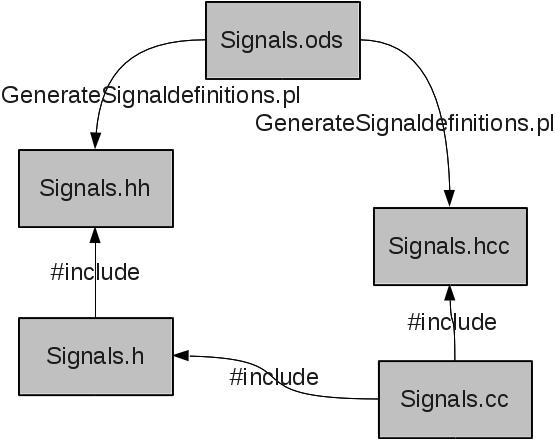
\includegraphics[width=10cm]{signals_ods.jpg}
\end{center}
\caption{Signal definitions by Spreadsheet}
\label{signals_ods}
\end{figure}

The generation is triggered by the plattform specific {\em Makefile}.
The script takes the desired target specifier(s) as command line
parameters.

\section{Signal Definition}
\label{sec_signal_definition}
The first sheet in {\em Signals.ods} contains the administrativ part.

\subsection{Grouping}
The signals are stored in groups. The definition of a group requires
an entry in the list of groups, which resides in the first sheet {\em GROUPS}
starting at line 3\footnote{This location must not be changed!}.
Each group entry consists of
\begin{description}
\item[Group name] which must have an identical name to the spreadsheet page.
   The sequence of spreadsheet pages must be identical to the sequence of
   group entries in this section.
\item[Group Number] defines the number region of the group.
    The {\em Group Number} is multiplied internally by 100.
    There may be 99 signals within each group.
\end{description}
The scripts checks for the matching of the group names and for multiple
usage of a group number.
The list of groups is terminated by an emtpy line.

\subsection{Groups}
Each group element contains the following entries:
\begin{description}
\item[GROUP INTERNAL ID] is the offset to the {\em Starting Number} of the 
   group. The id must be unique for all signals (not checked) to allow
   proper signal treatment by the runtime system.
   The {\em group internal id} 0 denotes the signal matching
   all signals defined in the group.
   The resulting signal {\em id} is created by the calculation of
   $GroupNumber \cdot 100 + GroupInternalId$
 
\item[ExceptionClass] defines the name of the C++ class, which shall be created.
   These names must by unique over all groups. This is also the name of
   the signal in the system part.
\item[ParentClass], which is used to build a C++ class hierarchy of the
    signals (C++ exceptions).
\item[System] specifies which plattform needs this signal. 
   The valid entries are defined by a drop down list. Please update the lists 
   on all sheets when a new plattform is added.
\item[Message] is the text which is sent to the standard output, when this
    signal was detected by the default signal handler.
\item[Description] contains the description of the reason for this signal
   for the external plattform signal manual. TeX syntax is allowed.
\end{description}

The scripts captures all entries of all group sheet with a matching
{\em System} entry.

\section{Decoration Scheme}
\begin{description}
\item[xxx] is the user supplied identifier for a signal
\item[theXxx] is t global identifier with the concrete signal object
\end{description}

\section{Usage in System Part}
A plattform specific signal is mapped to a user defined identifer in the 
system part. 
Each defined signal is statically instanciated to avoid
dynamic memory allocation when a exception should become thrown. 

\begin{PEARLCode}
CHAR_OVERFLOW: CharacterTooLongSignal;
\end{PEARLCode}

\begin{CppCode}
static pearlrt::Signal* _CHAR_OVERFLOW = pearlrt::theCharacterTooLongSignal;
\end{CppCode}

There is no possibility to define a signal upon its number, since this
produces lots of problems with the {\em static initialisation desaster}.
The identification of a signal at run time is done upon the signal id
which is referenced as {\em RST-value}.


\section{C++ Code for Signal Handler}
PEARL defines that a signal handler may be scheduled not inside 
a BEGIN/END-clause. The definition of a signal handler in a REPEAT block is also
prohibited. Thus we have access in the signal handler to all variables, which are defined
at the containing PROC or TASK level.
The definition of a signal handler inside of IF/THEN/ELSE-blocks is ok.

Possible reaction is a block of statements, which is executed and the
PROC is exited (the TASK teriminated) if the signal handler does not
contain a {\em GOTO-statement} defining the continuation point.
As extension to PEARL90 there a the possibility to \verb|INDUCE| the same, or another signal in OpenPEARL as signal reaction.
 
The language definition requires that a signal reaction will not triggered from inside the reation, thus a signal reaction must become disabled as soon as the
reaction becomes triggered.

The signal reactions ending with \verb|TERMINATE|, \verb|RETURN| do not require
to reenable the signal reaction, since the control flow ends with the statement.
In case of ending with an \verb|INDUCE| there might arise a problem of endless
loops between different signal reaction handlers. Thus the reaction must remain disabled when ending with \verb|INDIUCE|. 
The only case for enable a signal reaction arises with \verb|GOTO| from a signal handler into the application code.


Example:

\begin{PEARLCode}
SYSTEM;
   overfl: FixedOverFlowSignal;    
   div0:   FixedDivideByZeroSignal;
   arith:  ArithmeticSignal;

 PROBLEM;
   SPC overfl SIGNAL;
   SPC div0   SIGNAL;
   SPC arith  SIGNAL;

   X: PROC (p FIXED) 
      DCL k FIXED(15);

      k := 2;

restart: 
      ! signal action #1
      ON overfl BEGIN
         PUT 'PROC X: Arithmetic error (returning)' TO console BY A, SKIP;
         RETURN;
      END;

      ! signal action #2
      IF ( p == 1) THEN
         ON overfl BEGIN
            PUT 'PROC X: Overflow occured (terminating)' TO console BY A, SKIP;
            TERMINATE;     
         END;
      FIN;
      
      IF ( p > 5) THEN
      ! signal action #3
        ON overfl BEGIN
           PUT 'PROC X: Overflow occured (returning)' TO console BY A, SKIP;
           RETURN;
        END;
      FIN;

      ! signal action #4
      ON div0 BEGIN 
          PUT 'Divide by zero (restarting)' TO console BY A, SKIP;
          IF ( p ==  6) THEN
             GOTO EXIT;
          FIN;
          IF ( p = 11) THEN
              k:= 11//(k-k);   ! produce new div0 which is not caught again
          FIN;
          p := 6;
          GOTO RESTART;
      END;
      
      IF p == 11 THEN
          k := 10 // (k-k);  ! force 'div by 0'
      FIN;

      FOR i TO 100 REPEAT
        k := k * k;
      END;
exit:
  END;
\end{PEARLCode}

There are four signal handler defined in the procedure.
The \verb|Arithmetic| signal covers also the \verb|FixedOverFlowSignal|
and \verb|FixedDivideByZeroSignal| and some other error situations 
with arithmetics.

Since there are signals handler defined in the procedure,
the body is placed in a try-catch-block.
The catch block checks, whether the current signal matches 
on of the scheduled signal actions.

\begin{CppCode}
// system part
extern pearlrt::Signal *_overfl;
extern pearlrt::Signal * _div0;
extern pearlrt::Signal * _arith;

// problem part
SPCTASK(TASK1);

void _x(pearlrt::Task * me, pearlrt::Fixed<15> p) {
   pearlrt::Fixed<15> _k;

   //[ generated from ON statements in PROC
   pearlrt::SignalAction sigActions[5];
   pearlrt::ScheduledSignalActions scheduledSignalActions(5, sigActions);

    tryAgain:
    try {
       switch (indexOfSignalAction) {
          case -1: break;

       case 1: // first signal reaction
         ...
         break;

       } // end of switch
 
       // PROC or TASK body with schedudling of signal reactions
       ...  // normal code until first ON
      sigActions[1-1].setSignal(_artith);
      ...
      // 2nd ON
      sigActions[2-1].setSignal(_artith);
      ...
   } catch(pearlrt::Signal & s) {
       indexOfSignalAction = 
		scheduledSignalActions.getActionIndexAndSetRstAndDisableHandler(&s);
       if (indexOfSignalAction == 0) {
          // no handler found
          throw;
       }
       goto tryAgain; // signal handler found
    }
    // END OF SIGNAL FRAME
}  and of PROC or TASK
\end{CppCode}


Remarks:
\begin{description}
\item[disable signal handler] is done if the signal handler becomes
   active. Enabling is only necessray, if the handler is exited 
   with a GOTO statement, which requires a modified C++ code generation,
   when a GOTO statement leaves the range of a signal handler.
\item[sigActions] must be of type auto to provide task and procedure specific 
   signal reactions.
\end{description}

\section{C++ Code for Signal Handler with RST-Tag}
When a RST-element is specified in the ON-statement, the current
RST-value must be read into the given variable.

\begin{PEARLCode}
DCL Errorcode FIXED(15);
...
   ! version 1  ON statement in proc/task
   ON overfl RST(Errorcode): BEGIN .... END;

   ! version 2  ON statement in proc/task
   ON overfl RST(Errorcode);
\end{PEARLCode}

Version 1 is treated inside the function \verb|ScheduledSignalReactions::getActionIndexAndSetRstAndDisableHandler(Signal*s);|

Version 2 require that each statement in the task or procedure body ---
including the signal reactions --- becomes wrapped with a try catch block like:

\begin{CppCode}
    try {
       _x = CONST_FIXED_P_10_4;
    } catch (pearlrt::Signal & s) {
       scheduledSignalActions.setErrorOrThrow(&s);
    }
\end{CppCode}

This wrapping could be omitted for statements which do not 
throw a signal exception. This is part of a future check in the compiler.


\section{Induce}
The statement {\em INDUCE} simulates a signal and causes the trigger 
of the scheduled reaction.
Note that OpenPEARL forbids an induce statement with a RST-value.


\begin{PEARLCode}
INDUCE div_0;
\end{PEARLCode}

\begin{CppCode}
throw *_div_0;
\end{CppCode}

\section{Groups of Signals and Delegation of Signals to invoking Procedures and Task}


\begin{PEARLCode}
SYSTEM;
   TaskRunningSignal: TaskRunningSignal; ! number 102
   Arithmetic: ArithmethicSignal;        ! number 200

PROBLEM;
   SPC TaskRunningSignal SIGNAL;
   SPC Arithmetic SIGNAL;
   DCL Errorcode Fixed;
   DCL counter FIXED INIT(0);

Prog: TASK MAIN;
    ALL 1 SEC ACTIVATE Demo;
END;

Demo: TASK; 
   counter := counter + 1;

   ON TaskRunningSignal RST(ErrorCode)
	PUT 'TaskSignal occured with RST=', ErrorCode TO console BY A,F,SKIP;
   ON Arithimetic RST(ErrorCode)
	PUT 'Arithmetic problem occured with RST=', ErrorCode TO console BY A,F,SKIP;

   Test;
END;

Test: PROC;
   DCL k FIXED(15) INIT(2);

   CASE counter
   ALT /* 1 */ INDUCE TaskRunningSignal;
   ALT /* 2 */ k = k//(k-k);   ! produce divide by zero
   ALT /* 3 */ REPEAT  
	  	k = k * 2;  ! procuces FixedOverflowSignal
	       END;
   FIN;
END;
\end{PEARLCode}

This program will produce the output
\begin{verbatim}
TaskSignal occured with RST=200
Arithmetic problem occured with RST=102
Arithmetic problem occured with RST=103
\end{verbatim}

Sample C++ Code:
\begin{CppCode}
c++ code missing
\end{CppCode}
